\documentclass[a4paper, DIV12, headsepline]{scrartcl}

% common packages
\usepackage{lmodern}
\usepackage[T1]{fontenc}
\usepackage[utf8]{inputenc}
\usepackage[english]{babel}
\usepackage{amsfonts}
\usepackage{amssymb}
\usepackage{amsmath}
\usepackage{siunitx}
\usepackage{graphicx}
\usepackage{url}
\usepackage{listings}
\usepackage{tikz}
\usepackage{enumitem}
\usepackage[labelfont=bf]{caption}

% set head and foot
\usepackage{scrpage2}
\pagestyle{scrheadings}
\clearscrheadfoot
\ihead{Lab 2 -- Report}
\ohead{Group 25: Hui Jing (cid: huij), Tobias Fuchs (cid: fuchs)}
\cfoot{\pagemark}

% set pdf options
\usepackage[pdfborder={0 0 0}, bookmarksopen=true, bookmarksnumbered=true, pdftitle={Lab 2 Report}, pdfauthor={Hui Jing, Tobias Fuchs}, pdfsubject={Report}]{hyperref}

\begin{document}

\section*{Report for Lab 2}
\subsection*{Task 1}
For timing GEMM kernel, we use a scoped profiler to calculate the elapsed time of executing dot function and accumulate the execution time. The total time spent in dot function is printed out when the program exits.
\begin{verbatim}  
Run: time make run_pthreads  

dot exec time: 63889ms
real    1m6.346s
user    1m6.294s
sys     0m0.032s
\end{verbatim}
Percentage of dot execution: 63.889/66.346 = 96.2967\%

\subsection*{Task 2}
\begin{enumerate}[label=\alph*)]
\item We have applied the loop permutation technique to achieve a more locality preserving access. To be more specific, we have reordered the loops in the following way.
\begin{verbatim}
for (int row = 0; row < m1_rows; ++row)
  for (int k = 0; k < m1_columns; ++k)
    for (int col = 0; col < m2_columns; ++col)
      output[row * m2_columns + col] += ...;
\end{verbatim}

\item Before the transformation, the total running time is \SI{67.508550}{s}, whereby the running time of the \texttt{dot} function is \SI{64.991598}{s} (\SI{96.271654}{\%} of total running time). After the transformation, the total running time is \SI{10.498188}{s}, whereby the running of the \texttt{dot} function is \SI{7.994576}{s} (\SI{76.151964}{\%} of total running time). The amount of running time that is spent in the \texttt{dot} function has been reduced significant from \SI{96.271654}{\%} to \SI{76.151964}{\%} (difference \SI{20.11969}{\%}).
\end{enumerate}

% for (int row = 0; row < m1_rows; ++row)
%   for (int k = 0; k < m1_columns; ++k)
%     for (int col = 0; col < m2_columns; ++col)
%       output[row * m2_columns + col] += m1[row * m1_columns + k] * m2[k * m2_columns + col];

% Total time in dot: 7.994576s
% Total time for all: 10.498188s
% of running time in dot: 76.151964%

\subsection*{Task 3}
\begin{enumerate}[label=\alph*)]
\item The cache line size of the machine is 64 bytes by "getconf -a | grep CACHE". Theoretically, we shall get the best performance if BLOCK\_SIZE * sizeof(float) equals to a cache line size, i.e. const int block\_size = 64 / sizeof(float);

\item Our implementation of loop tiling:
\begin{verbatim}  
    int N = m1_rows;
    int M = m1_columns;
    int K = m2_columns;
    for (int i0 = 0; i0 < N; i0 += block_size) {
        int imax = i0 + block_size > N ? N : i0 + block_size;
        for (int j0 = 0; j0 < M; j0 += block_size) {
            int jmax = j0 + block_size > M ? M : j0 + block_size;
            for (int k0 = 0; k0 < K; k0 += block_size) {
                int kmax = k0 + block_size > K ? K : k0 + block_size;
                for (int j1 = j0; j1 < jmax; ++j1) {
                    int sj = K * j1;
                    for (int i1 = i0; i1 < imax; ++i1) {
                        int mi = M * i1;
                        int ki = K * i1;
                        for (int k1 = k0; k1 < kmax; ++k1) {
                            output[ki + k1] += m1[mi + j1] * m2[sj + k1];
     }}}}}}
\end{verbatim}
\item We have observed that BLOCK\_SIZE < 64 is not as good as BLOCK\_SIZE = 64. However, if we use task2 result as baseline, loop tiling didn´t significantly improve the cache hit. This could be explained by that the float vector is not aligned with cache line size, which causes extra cache miss even with looping technique. Meanwhile, extra loop instructions also increase the total execution time. In summary, we got better cache hits, but the total execution time increased.

%When we increase the BLOCK\_SIZE, the result is getting closer and closer to the one %obtained in task2. Of course, when the BLOCK\_SIZE is big enough, the implementation is %identical to task2 implementation.

Below is the result of baseline and loop tiling with BLOCK\_SIZE = 64:

\begin{verbatim}  
Run: perf stat --repeat 10 -e LLC-load-misses ./nnetwork

 Performance counter stats for './nnetwork' (10 runs):
      Baseline:
           441,399      LLC-load-misses:u                                             ( +-  3.38% )
          10.47281 +- 0.00513 seconds time elapsed  ( +-  0.05% )

      Loop tiling:
           415,132      LLC-load-misses:u                                             ( +-  2.12% )
           16.6134 +- 0.0106 seconds time elapsed  ( +-  0.06% )
\end{verbatim}

\end{enumerate}
% Before:
% Performance counter stats for './nnetwork':
%
%           511,665      LLC-load-misses:u                                           
%
%      10.513226493 seconds time elapsed
%
%      10.466333000 seconds user
%       0.039978000 seconds sys

\subsection*{Task 4}
\begin{enumerate}[label=\alph*)]
\item The following snippet shows our implementation of the parallel version of the \textsc{Gemm} kernel.
\begin{verbatim}
...

const int chunk = m1_rows / num_partitions;
const int remainder = m1_rows % num_partitions;

pthread_t threads[num_partitions];

for (int i = 0; i < num_partitions; ++i)
{
  gemm_thread_args *args = new gemm_thread_args;

  args->m1 = &m1;
  args->m1_columns = m1_columns;
  args->m1_rows = m1_rows;
  args->m2 = &m2;
  args->m2_columns = m2_columns;
  args->output = &output;

  args->row_start = i * chunk + std::min(i, remainder);
  args->row_end = (i + 1) * chunk + std::min(i + 1, remainder);

  pthread_create(&threads[i], NULL, &dot_block, args);
}

for (int i = 0; i < num_partitions; ++i)
  pthread_join(threads[i], NULL);

...
\end{verbatim}

\item The running times for different number of threads are given by the table below.
\begin{table}[htbp]
\centering
\sisetup{table-number-alignment=left,table-format=3.6,table-auto-round}
\begin{tabular}{cS}
\hline
{Number of threads} & {Total running time (s)} \\
\hline
1 & 133.080872 \\
2 & 70.213904 \\
4 & 38.302974 \\
8 & 38.577283 \\
16 & 39.085463 \\
32 & 40.197144 \\
64 & 42.522234 \\
\hline
\end{tabular}
\end{table}

\item Since the used computer has 4 processor cores, the usage of more than 4 threads does not yield any improvement. Using more than 4 threads leads to an increasing total running time because the overhead for the thread management becomes larger and the maximum number of threads that can be executed in parallel stays constant.

\end{enumerate}

% 1 Thread
% Total time in dot: 130.487245s
% Total time for all: 133.080872s
% % of running time in dot: 98.051089%

% 2 Threads
% Total time in dot: 67.654698s
% Total time for all: 70.213904s
% % of running time in dot: 96.355129%

% 4 Threads
% Total time in dot: 35.699967s
% Total time for all: 38.302974s
% % of running time in dot: 93.204166%

% 8 Threads
% Total time in dot: 36.038386s
% Total time for all: 38.577283s
% % of running time in dot: 93.418671%

% 16 Threads
% Total time in dot: 36.522703s
% Total time for all: 39.085463s
% % of running time in dot: 93.443189%

% 32 Threads
% Total time in dot: 37.582485s
% Total time for all: 40.197144s
% % of running time in dot: 93.495412%

% 64 Threads
% Total time in dot: 39.881794s
% Total time for all: 42.522234s
% % of running time in dot: 93.790447%

\subsection*{Task 5}
\begin{enumerate}[label=\alph*)]
\item Besides the multi-threading implementation, we also did loop interchange to improve the performance. 

When the program run with 1 processor, total execution time: 

11.786s = 2.605(sequential) + 9.181(parallelizable)

If assume linear speedup, considering the machine has 4 cores, the theoretical  maximum speedup can be achieved is: 11.786/(2.605 + 9.181/4) = 2.41

\item We used 1,2,3,4 threads to train the network respectively. 

Sequential part: 

	    2.605s (1 thread), 2.558s (2 threads), 2.605s (3 threads), 2.591s (4 threads)

Parallel part: 

	    9.181s (1 thread), 4.777s (2 threads), 3.499s (3 threads), 2.711s (4 threads)

\begin{center}
	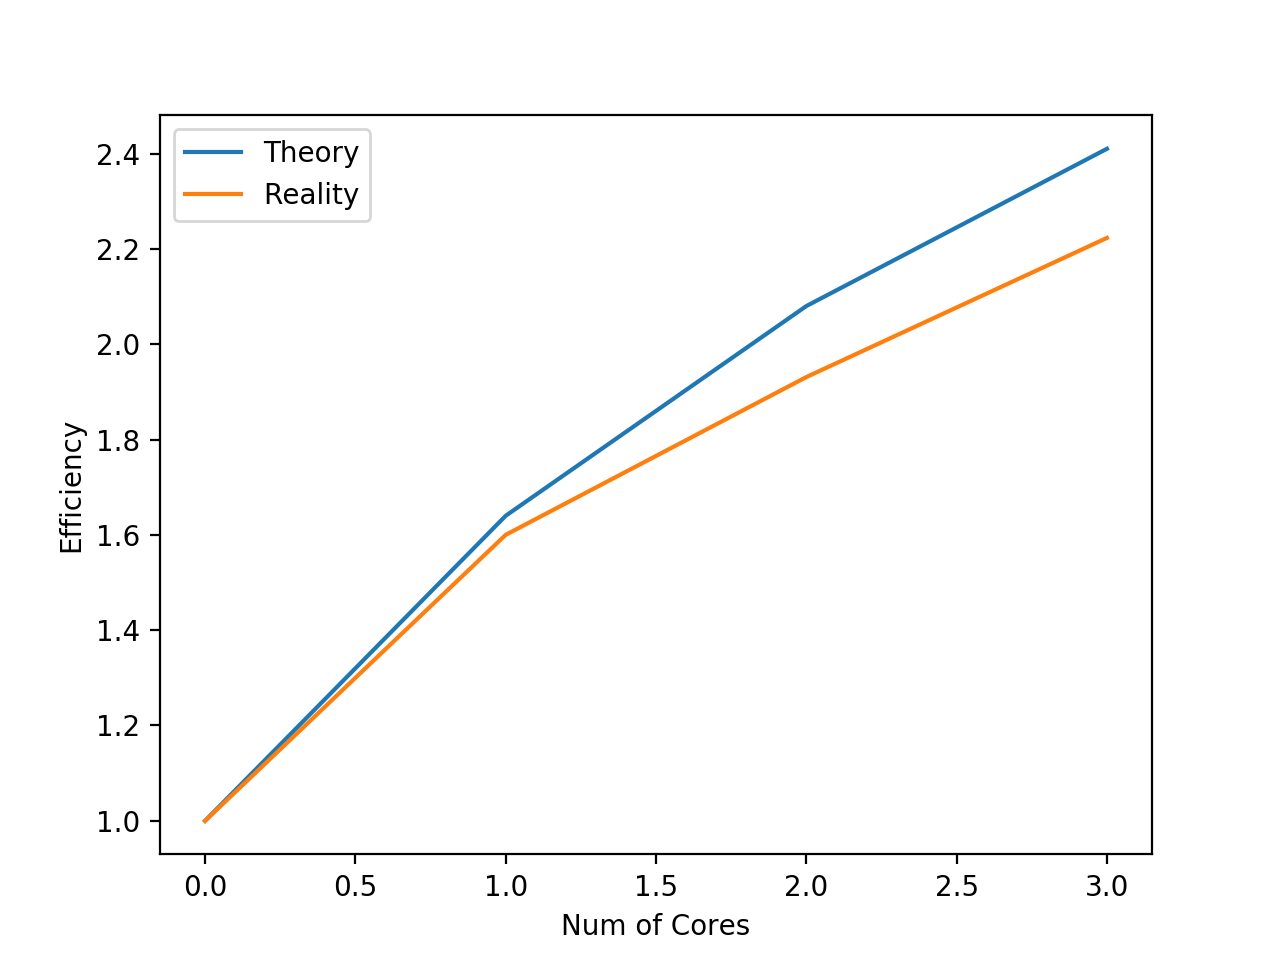
\includegraphics[scale=0.5]{task-5-plot}
\end{center}

%theoretical:	    
%11.786/(2.605 + 9.181/4) = 2.41
%11.786/(2.605 + 9.181/3) = 2.08
%11.786/(2.605 + 9.181/2) = 1.64
%11.786/(2.605 + 9.181/1) = 1
%
%reality:
%11.786/(2.591 + 2.711) = 2.223
%11.786/(2.605 + 3.499) = 1.931
%11.786/(2.558 + 4.777) = 1.60
%11.786/(2.605 + 9.181) = 1

\item The efficiency that we achieved with 4 threads is : 11.786/(2.591 + 4*2.711) = 0.877
%dot exec time: 9181ms
%real    0m11.786s
%user    0m11.531s
%sys     0m0.231s
%
%dot exec time: 4777ms
%real    0m7.335s
%user    0m11.546s
%sys     0m0.233s
%
%dot exec time: 3499ms
%real    0m6.104s
%user    0m11.858s
%sys     0m0.321s
%
%dot exec time: 2711ms
%real    0m5.302s
%user    0m11.539s
%sys     0m0.435s
\end{enumerate}
%  3.728% not par. (time not in dot) -> max speed up 26.822, with 4 processors max spped up 3.598
%  5% not parallelizable -> max speed up 20, with 4 processors max speed up 3.478
% 25% not parallelizable -> max speed up  4, with 4 processors max speed up 2.286

\end{document}
